%& --translate-file latin2pl
\documentclass{article}

\usepackage{polski}
\usepackage{hyperref}
\usepackage[T1]{fontenc}
\usepackage[utf8]{inputenc}
\usepackage{listings}
\hypersetup{
colorlinks=true,
urlcolor=blue,
}

\lstset{
basicstyle=\fontsize{6}{6}\selectfont\ttfamily,
}
\usepackage{graphicx}
\graphicspath{ {./images/} }
\usepackage[dvipsnames]{xcolor}

\definecolor{kolorAdministracyjna}{RGB}{255, 153, 153}
\definecolor{kolorZarzad}{RGB}{179, 255, 102}
\definecolor{kolorPrawny}{RGB}{255, 153, 51}
\definecolor{kolorProgramistyczny}{RGB}{51, 255, 255}
\definecolor{kolorGraficzny}{RGB}{255, 51, 255}
\definecolor{kolorKsiegowy}{RGB}{204, 204, 0}
\definecolor{kolorGoscinna}{RGB}{153, 0, 77}

\title{SIK\\Zadanie 3}
\author{Marcin Abramowicz ma406058}


\begin{document}
  \maketitle

  \section{Ogólny opis}
    Budynek A jest połączony ze światem zewnętrznym przez router z firewallem. W każdym budnyku znajduje się "duży" switch, który po swiatłowodzie jest podłączony złączem VLAN Trunk z "dużymi" switchami pozostałych budynków. Muszą one wspierać STP, aby nie powstawały pętle, natomiast w razie awarii jednego ze światłowodów komunikacja mogła przebiegać działającymi. Każdy z nich wewnątrz swojego budynku udostępnia podsieci potrzebne dla pracowników, są one podłączone do odpowiednich portów w tym switchu. Aby zapewnić dostęp do internetu gościom oraz umożliwić pracownikom wymianę informacji między działami firmy dodatkowo istnieją odpowiednio podsieć gościnna i administracyjna.

    \centerline{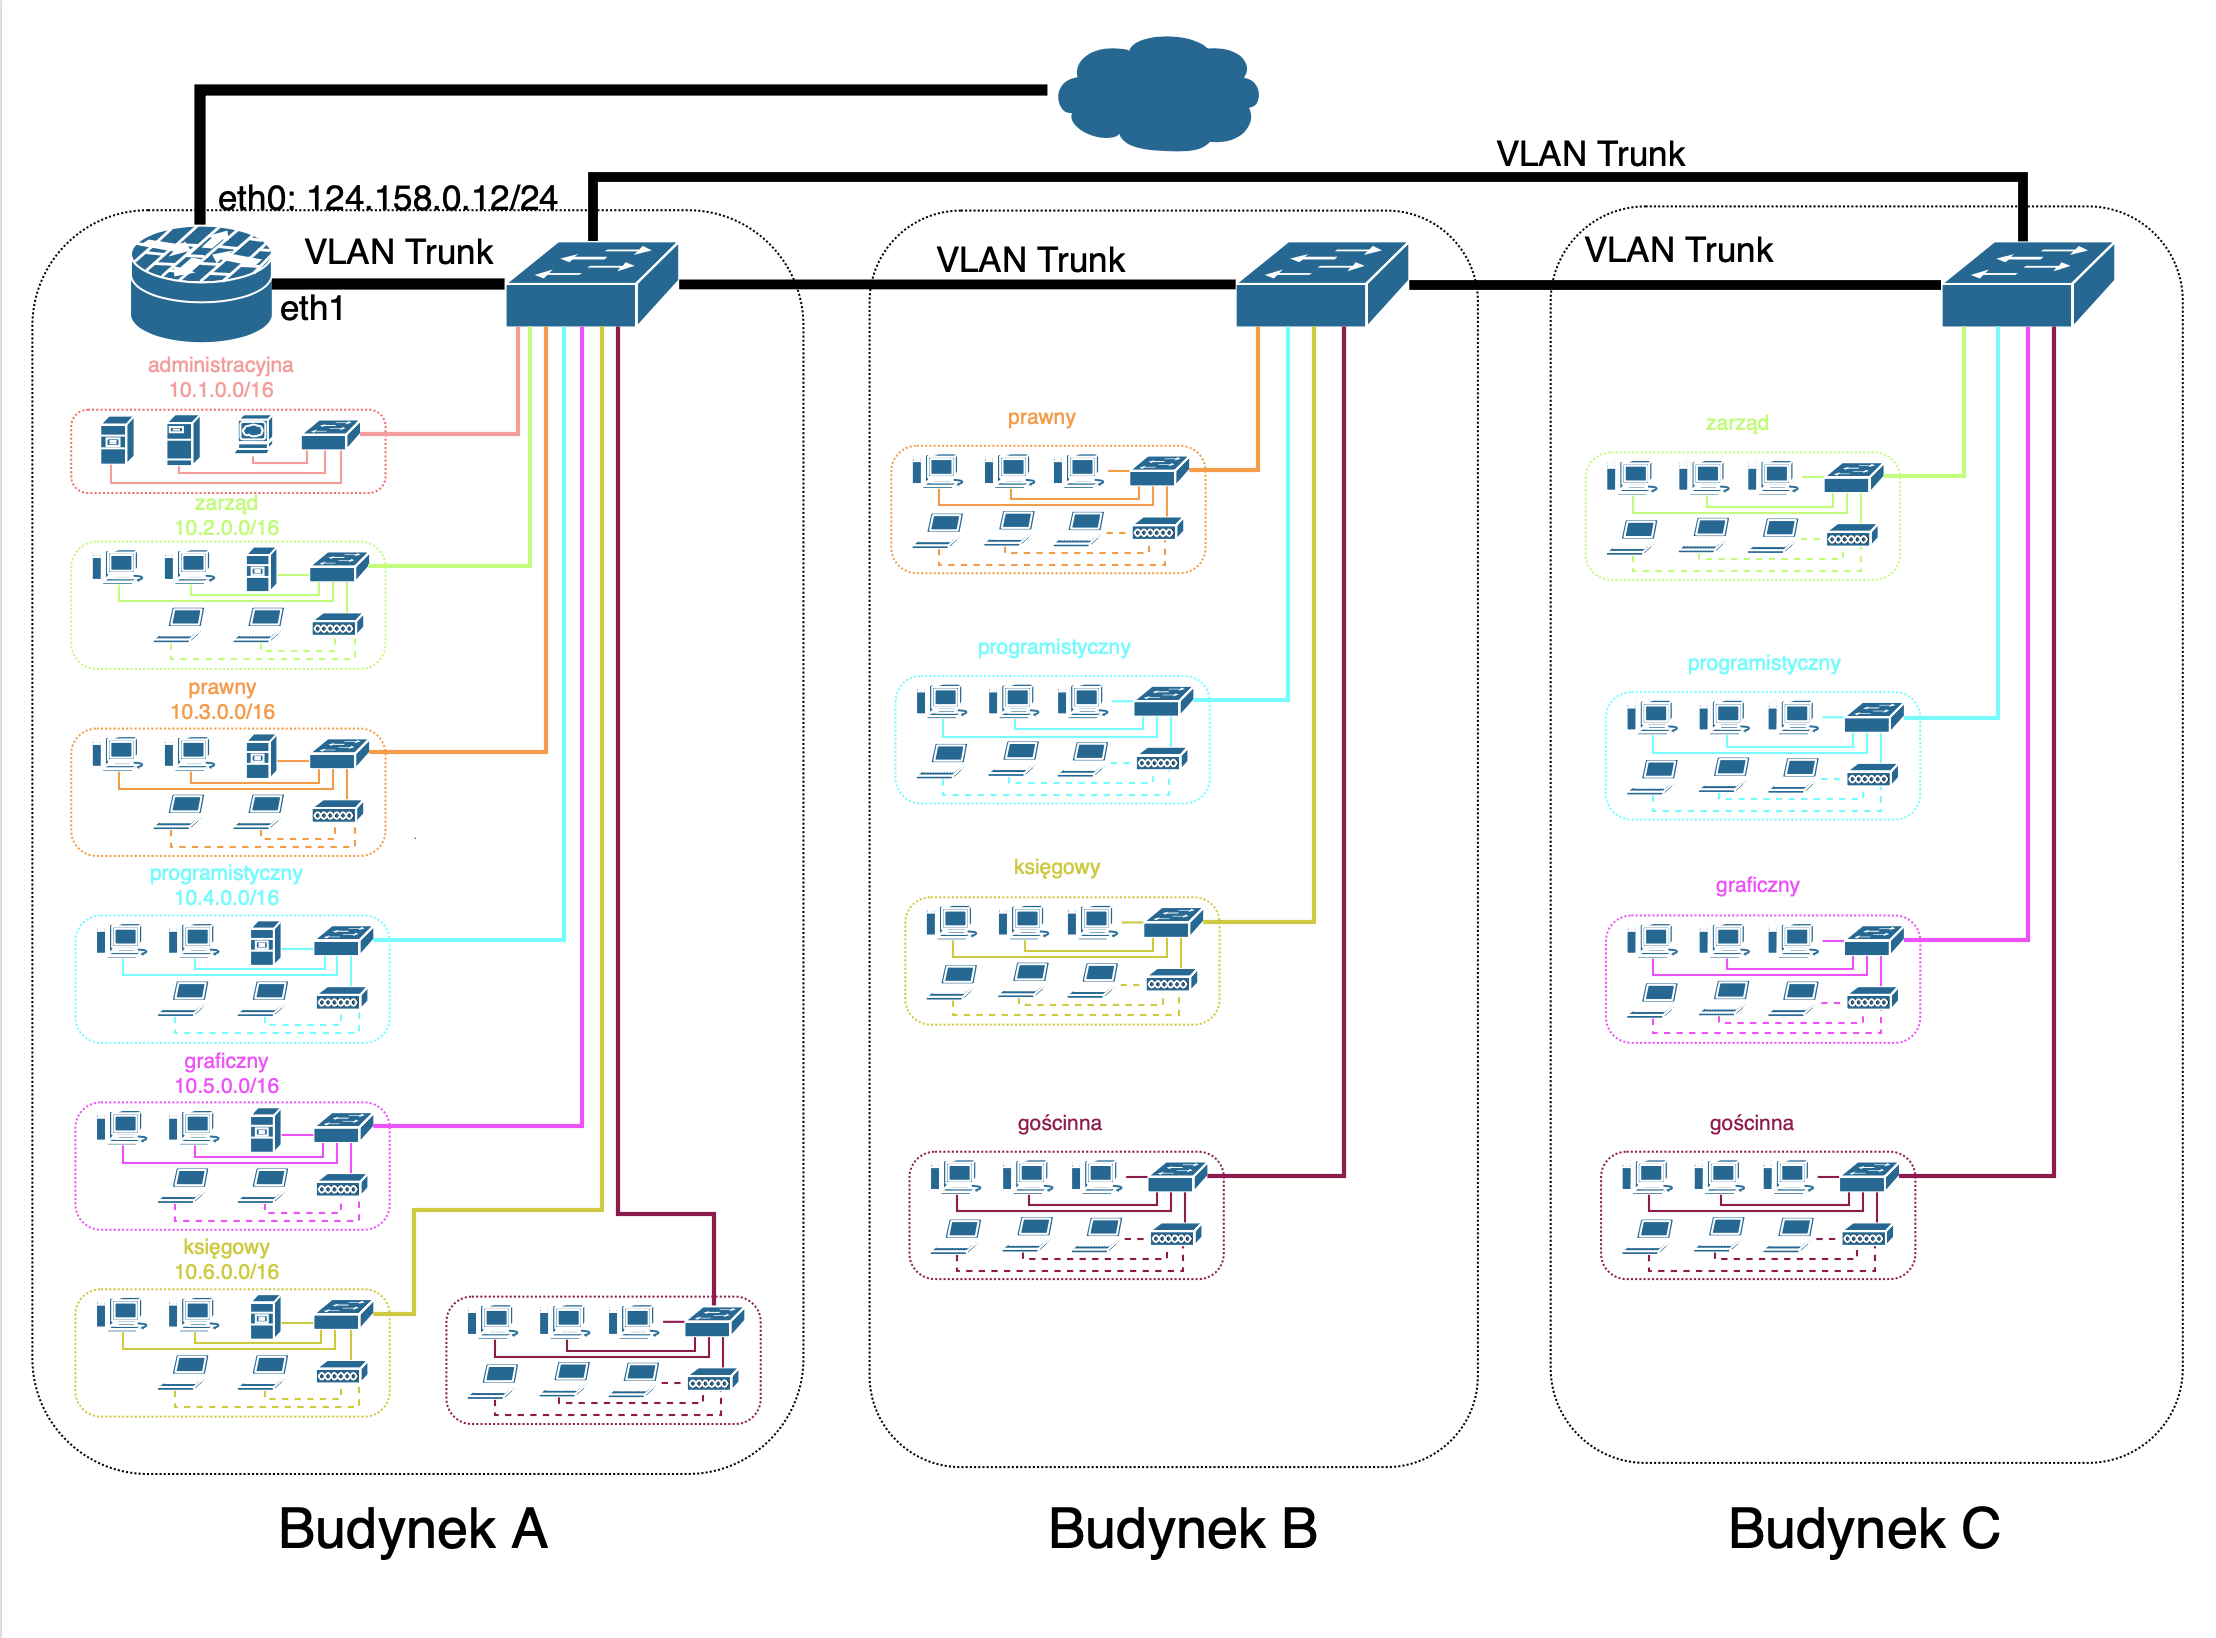
\includegraphics[width=\paperwidth,keepaspectratio]{schemat-sieci}}


  \section{Podsieci}
    Dla rozróżnienia przeznaczenia identyfikatory VLAN zaczynajęce się od 1 są administracyjne, od 2 - działy firmy, 3 - gościnne.
    \subsection{Podsieć administracyjna}
      \begin{tabular}{|c|c|c|}
        Nazwa & VLAN id & Podsieć \\
        \hline
        \textcolor{kolorAdministracyjna}{administracyjna} & \textcolor{kolorAdministracyjna}{11} & \textcolor{kolorAdministracyjna}{10.1.0.0/16} \\
      \end{tabular}

    \subsection{Podsieci działów}
      \begin{tabular}{|c|c|c|}
        Nazwa działu& VLAN id & Podsieć \\
        \hline
        \textcolor{kolorZarzad}{zarząd} & \textcolor{kolorZarzad}{22} & \textcolor{kolorZarzad}{10.2.0.0/16} \\
        \hline
        \textcolor{kolorPrawny}{prawny} & \textcolor{kolorPrawny}{23} & \textcolor{kolorPrawny}{10.3.0.0/16} \\
        \hline
        \textcolor{kolorProgramistyczny}{programistyczny} & \textcolor{kolorProgramistyczny}{24} & \textcolor{kolorProgramistyczny}{10.4.0.0/16} \\
        \hline
        \textcolor{kolorGraficzny}{graficzny} & \textcolor{kolorGraficzny}{25} & \textcolor{kolorGraficzny}{10.5.0.0/16} \\
        \hline
        \textcolor{kolorKsiegowy}{księgowy} & \textcolor{kolorKsiegowy}{26} & \textcolor{kolorKsiegowy}{10.6.0.0/16} \\
      \end{tabular}

    \subsection{Podsieć gościnna}
      \begin{tabular}{|c|c|c|}
        Nazwa & VLAN id & Podsieć \\
        \hline
        \textcolor{kolorGoscinna}{gościnna} & \textcolor{kolorGoscinna}{37} & \textcolor{kolorGoscinna}{10.7.0.0/16} \\
      \end{tabular}

  \section{Opis pojedyńczych podsieci}
    \subsection{Podsieć administracyjna}
      \centerline{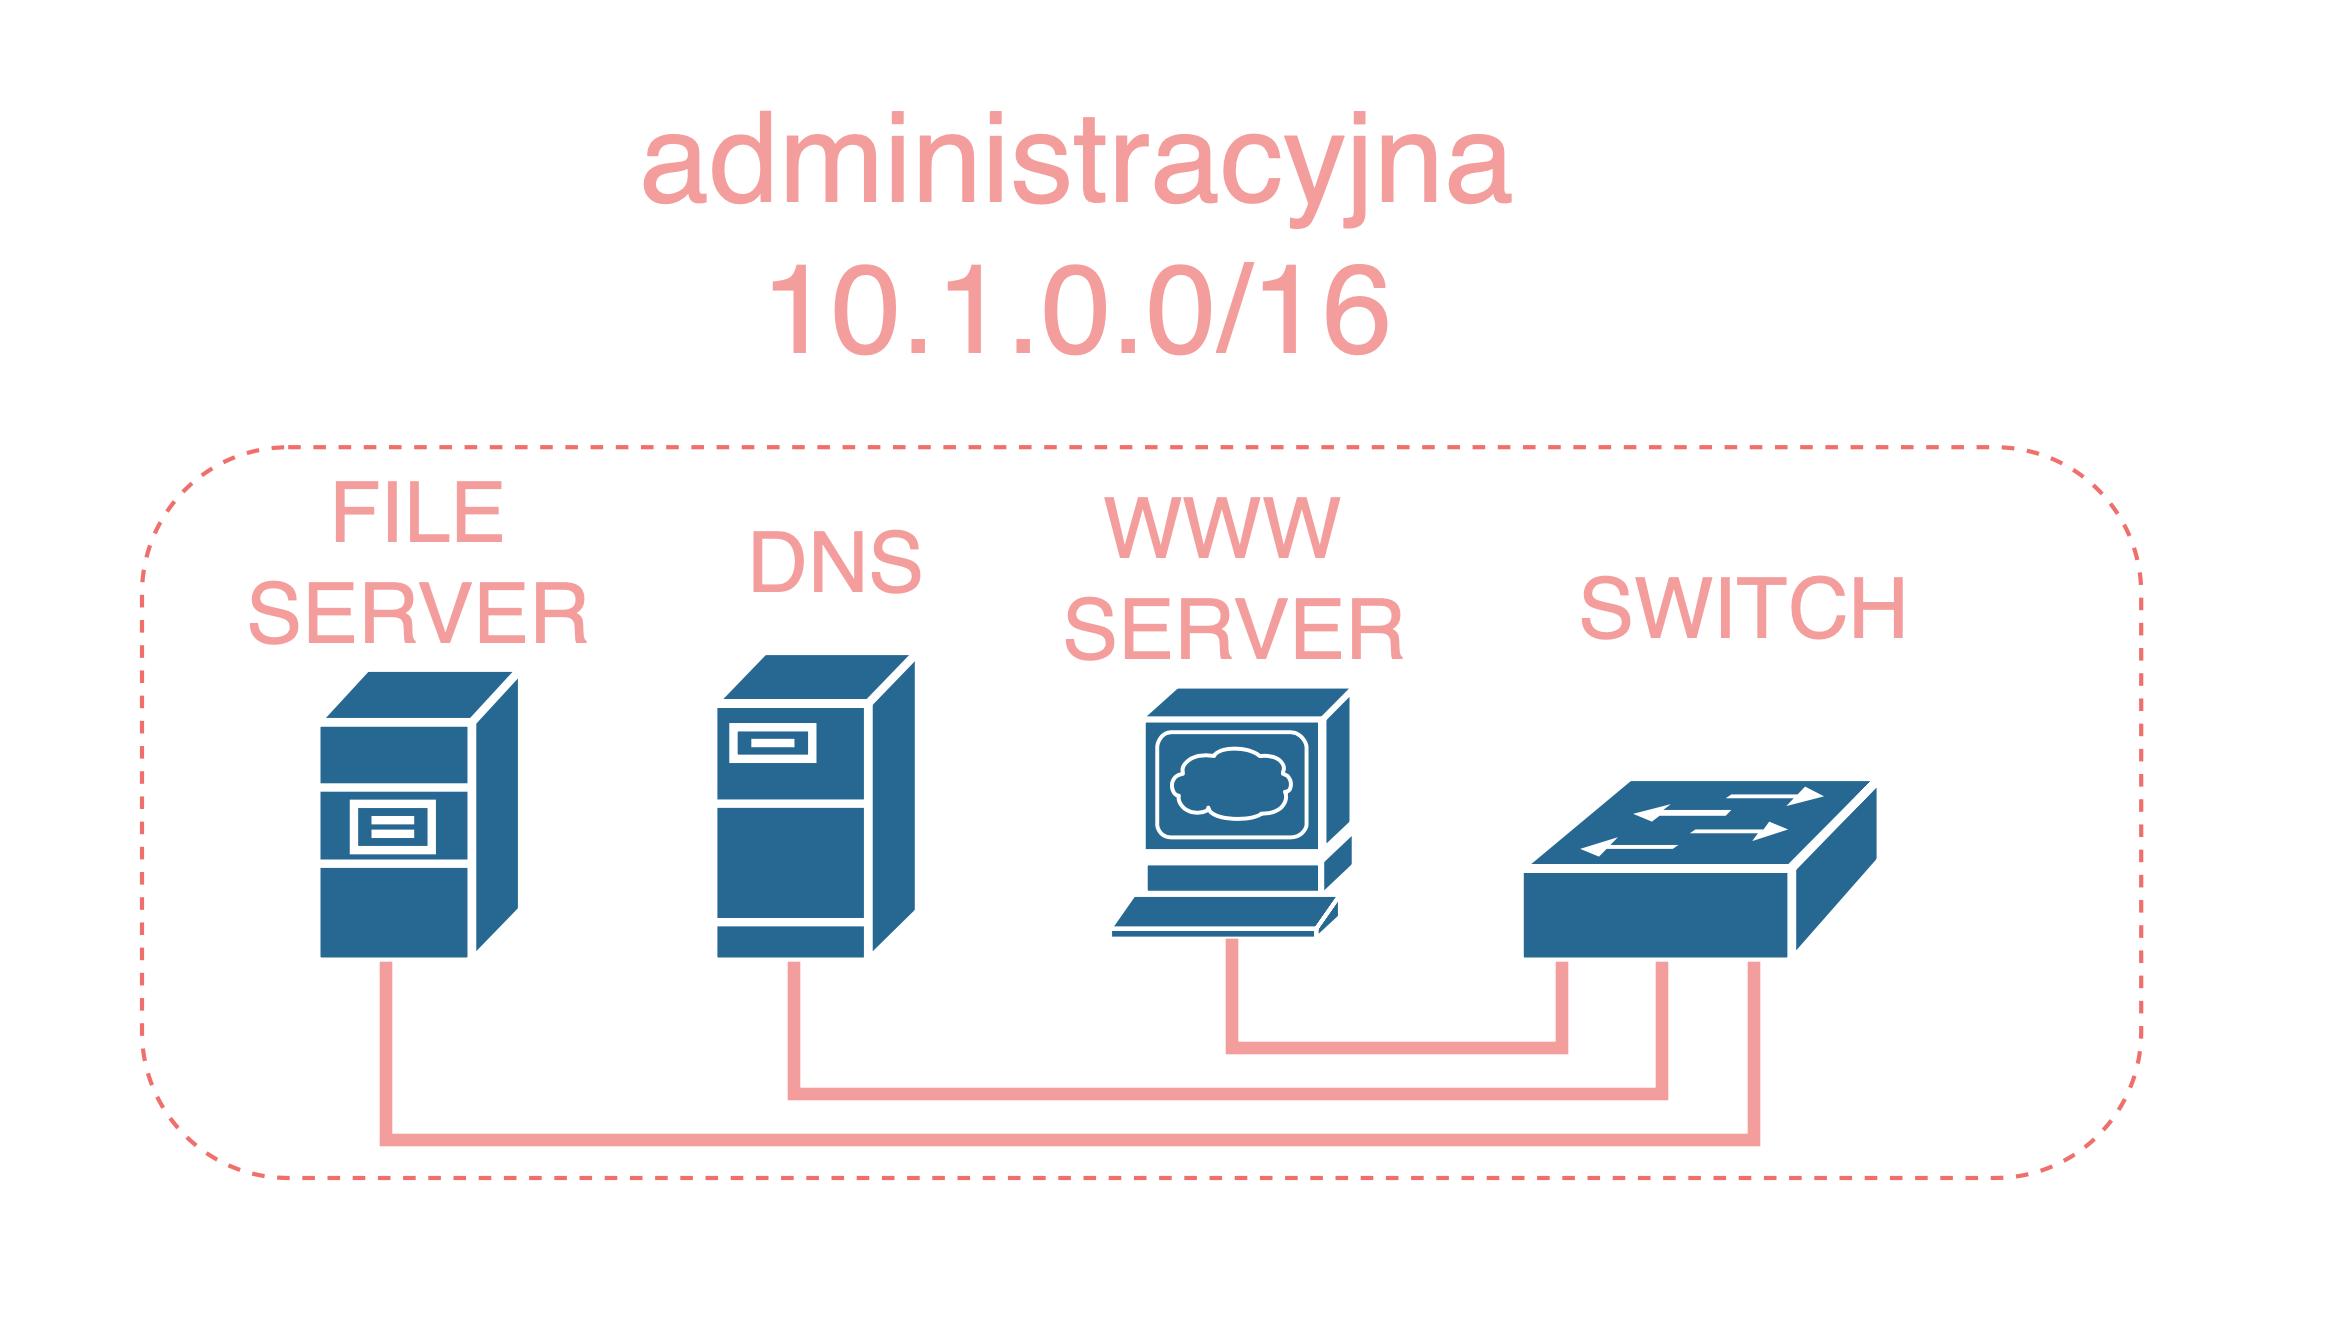
\includegraphics[width=\textwidth,keepaspectratio]{podsiec-administracyjna}}

      Znajduje się ona w budynku A.
      Składa się ona z "małego" switcha, jest on podłączony do "dużego" do odpowiedniego portu.
      Znajduje się w niej serwer plików, do którego maja dostęp pracownicy wszystkich działów firmy, umożliwia wymiane plików między nimi.
      Posiada również serwer WWW, dzięki któremu firma będzie mogła posiadać stronę WWW oraz serwer DNS do wewnętrznego użycia.

    \subsection{Podsieci działów}
      Podsieci działów podzielimy, na te które znajdują się w budnyku A i posiadają serwery dla danej podsieci oraz na te w pozostałych budynkach, bez własnych serwerów, używających serwera z budynku A. Umożliwi to swobodną wymianę danych wewnątrz działu, tak aby inne działy nie miały dostępu do tych danych.

      \subsubsection{Podsieci działów w budynku A}
        Przykład dla zarządu.

        \centerline{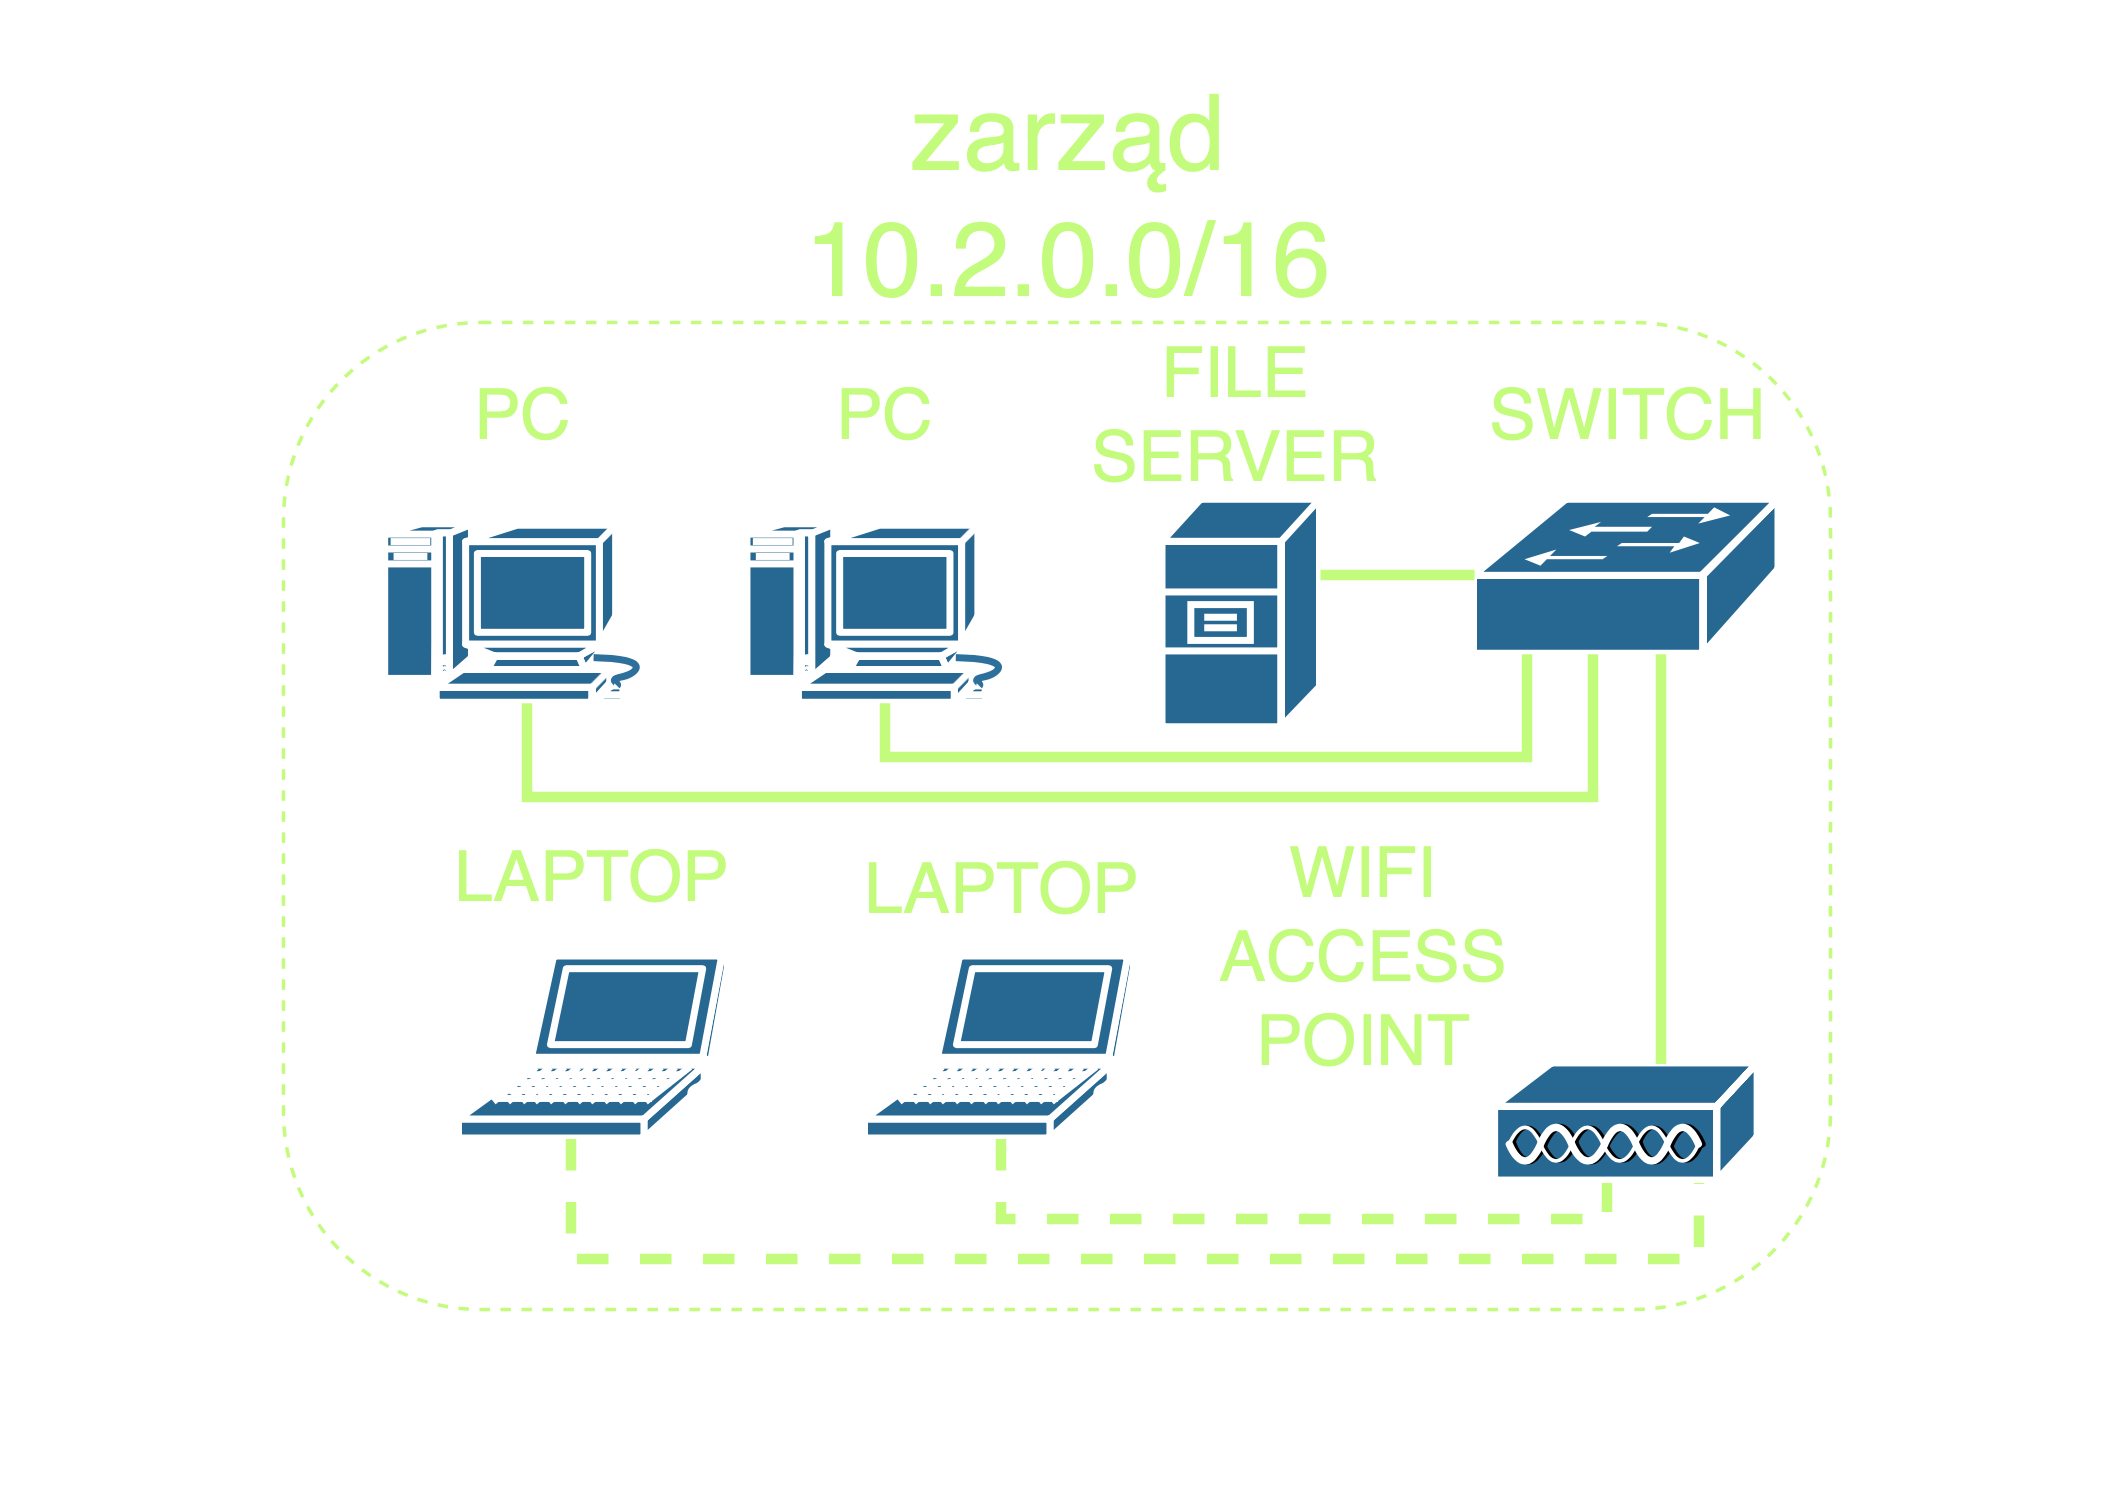
\includegraphics[width=\textwidth,keepaspectratio]{podsiec-zarzad-z-serwerem}}

        Składa się ona również z "małego" switcha, podłaczonego do "dużego" w budynku A.
        Posiada serwer plików, aby każdy dział mógł wymieniać się danymi.
        Podłączone są do niej komputery pracowników oraz access point umożliwiający bezprzewodowe podłączenie się do niej z laptopów i urządzeń mobilnych (oczywiście logowanie powinno wymagać loginu i hasła od pracownika).

      \subsubsection{Podsieci działów w budynkach B i C}
        Przykład dla działu prawnego.
        
        \centerline{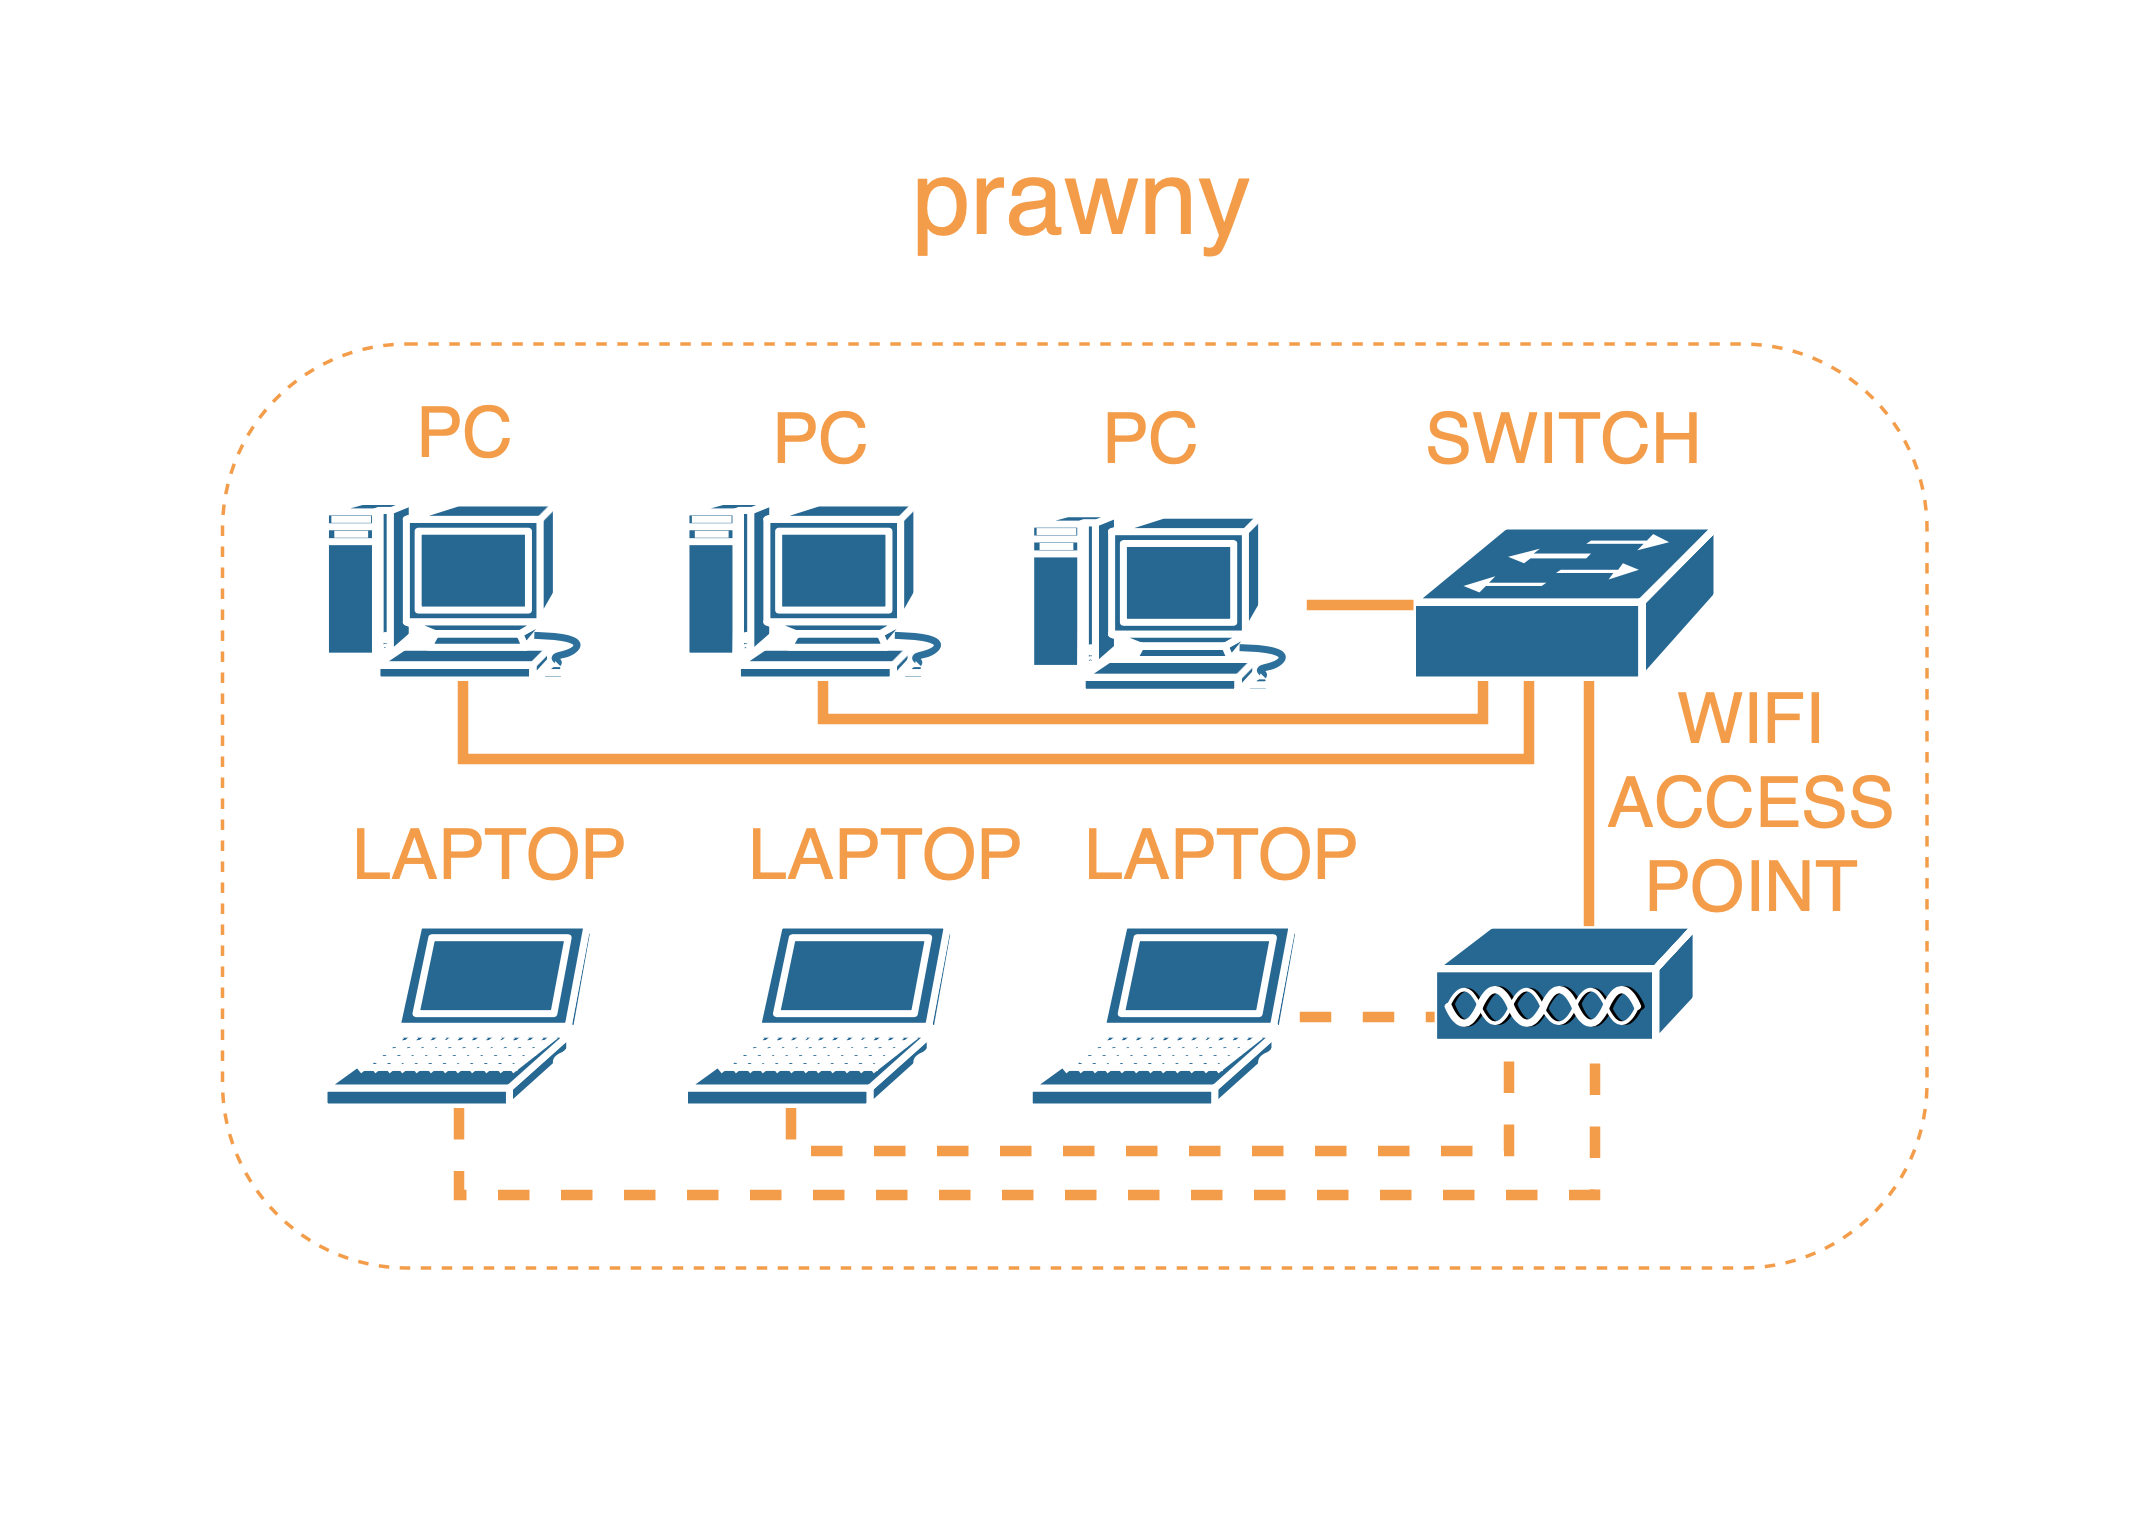
\includegraphics[width=\textwidth,keepaspectratio]{podsiec-prawny-bez-serwera}}

        Składa się ona również z "małego" switcha, podłaczonego do "dużego" w ich budynku.
        Podłączone są do niej jedynie komputery pracowników oraz access point umożliwiający bezprzewodowe podłączenie się do niej z laptopów i urządzeń mobilnych (oczywiście logowanie powinno wymagać loginu i hasła od pracownika).
        Wymiana plikami odbywa się poprzez serwer umieszczony w budynku A dla danej podsieci.

    \subsection{Podsieć gościnna}
      Goście mogą korzystać z własnej podsieci, nie posiada ona serwera plików (goście nie powinni potrzebować), a jedynie z komputerów (na przykład na parterze) oraz bezprzewodowego access pointu i aby się do niej zalogować gość powinien podać hasło.


  \section{Tablica tras routera}
    \begin{tabular}{|c|c|c|c|}
      cel & maska & interface & brama \\
      \hline
      \textcolor{kolorAdministracyjna}{10.1.0.0} & \textcolor{kolorAdministracyjna}{255.255.0.0} & \textcolor{kolorAdministracyjna}{eth1/11} & \textcolor{kolorAdministracyjna}{0.0.0.0} \\
      \hline
      \textcolor{kolorZarzad}{10.2.0.0} & \textcolor{kolorZarzad}{255.255.0.0} & \textcolor{kolorZarzad}{eth1/22} & \textcolor{kolorZarzad}{0.0.0.0} \\
      \hline
      \textcolor{kolorPrawny}{10.3.0.0} & \textcolor{kolorPrawny}{255.255.0.0} & \textcolor{kolorPrawny}{eth1/23} & \textcolor{kolorPrawny}{0.0.0.0} \\
      \hline
      \textcolor{kolorProgramistyczny}{10.4.0.0} & \textcolor{kolorProgramistyczny}{255.255.0.0} & \textcolor{kolorProgramistyczny}{eth1/24} & \textcolor{kolorProgramistyczny}{0.0.0.0} \\
      \hline
      \textcolor{kolorGraficzny}{10.5.0.0} & \textcolor{kolorGraficzny}{255.255.0.0} & \textcolor{kolorGraficzny}{eth1/25} & \textcolor{kolorGraficzny}{0.0.0.0} \\
      \hline
      \textcolor{kolorKsiegowy}{10.6.0.0} & \textcolor{kolorKsiegowy}{255.255.0.0} & \textcolor{kolorKsiegowy}{eth1/26} & \textcolor{kolorKsiegowy}{0.0.0.0} \\
      \hline
      \textcolor{kolorGoscinna}{10.7.0.0} & \textcolor{kolorGoscinna}{255.255.0.0} & \textcolor{kolorGoscinna}{eth1/37} & \textcolor{kolorGoscinna}{0.0.0.0} \\
      \hline
      0.0.0.0 & 0.0.0.0 & eth0 & 124.158.0.23 \\
    \end{tabular}


  \section{Przydzielanie adresów IP}
    Router na interface eth1 ma serwer DHCP, który dla wybranych urządzeń (rozpoznawanych po adresie MAC), żeby można było używać ich usług, przydziela zawsze ten sam adres IP.
    Dla serwerów w każdej podsieci przypisuje zawsze ten sam adres: \\
    10.<podsieć>.0.1

    Dodatkowo dla urządzeń w \textcolor{kolorAdministracyjna}{podsieci administracyjnej}, przydziela następujące adresy: \\
    - serwer DNS - \textcolor{kolorAdministracyjna}{10.1.0.2} \\
    - serwer WWW - \textcolor{kolorAdministracyjna}{10.1.0.3}


  \section{Reguły NAT}
    Router ma jedynie otwarte porty do protokołów HTTP i HTTPS - 80, 443, które to są mapowane na odpowiednie porty serwera WWW (\textcolor{kolorAdministracyjna}{10.1.0.3}) z \textcolor{kolorAdministracyjna}{podsieci administracyjnej}.


  \section{Firewall routera}
    Firewall routera w budynku jest ustawiony tak, aby blokować komunikację między: \\
    - VLANem podsieci gościnnej, pozostałymi podsieciami (administracyjna, działowe) \\
    - VLANami podsieci działów (między działami, do podsieci administracyjnej komunikacja ma nie być blokowana). \\
    Firewall blokuje wszystkie przychodzące połączenia ze świata zewnętrznego, ale pozwala na połączenia wychodzące.



  \section{Potrzebny sprzęt}
    - 1 router (z DHCP, firewallem) \\
    - 3 switche (z VLAN, STP) \\
    - 15 switchy (zwykłe) \\
    - 14 access pointów \\
    - maszyna serwerowa pod serwer WWW \\
    - maszyna serwerowa pod serwer DNS \\
    - 6 maszyn serwerowych pod serwery dla każdej podsieci


  \section{Wypełnienie wymagań}
    \subsection{W każdym budynku należy zapewnić dostęp do Internetu także dla gości firmy}
      Każda podsieć może połączyć się do internetu, ponieważ firewall nie blokuje takich połączeń.
      Pracownicy i gości mogą to uczynić komputerami kablowo podłączonymi do switcha lub bezprzewodowo dzieki access pointom.

    \subsection{W każdym budynku powinna być zainstalowana sieć przewodowa zbudowana na bazie Ethernetu i sieć bezprzewodowa zbudowana na bazie Wi-Fi}
      Każda podsieć posiada sieć Ethernet podłączoną bezpośrednio do "małych" switchy oraz sieć Wi-Fi dzięki bezprzewodowym access pointom.

    \subsection{Fragmenty sieci przewodowej używane przez zarząd powinny być szczególnie chronione przed dostępem z zewnątrz}
      Sieć zarządu, podobnie jak wszystie pozostałe, są chronione regułami firewall przed dostępem z zewnątrz.

    \subsection{Każdy z działów powinien mieć możliwość udostępniania danych dostępnych tylko dla pracowników danego działu a niedostępnych dla pracowników innych  działów w firmie}
      Każdy dział używając własnej podsieci może udostępniać dane tylko dla pracowników tego działu, tym samym nie dając możliwości dostępu do nich z zewnątrz.

    \subsection{Powinna być także możliwość udostępniania pewnych danych wszystkim pracownikom firmy w taki sposób by nie były one dostępne bezpośrednio z sieci zewnętrznej}
      Dzięki serwerowi w sieci administracyjnej, do której dostęp maja wszyscy pracownicy firmy, można udostępniać dane dla całej firmy, a uniemożliwiając dostęp do nich z zewnątrz.

    \subsection{Firma będzie chciała udostępniać własny serwis WWW}
      W sieci administracyjnej jest odpowiedni serwer WWW, który dzięki regułom NAT umożliwi udostępnianie własnej strony WWW.

    \subsection{Poszczególne działy firmy potrzebują serwerów z różnego rodzaju oprogramowaniem: systemem zarządzania projektami, bazą danych, repozytorium}
      Każdy dział posiada własny serwer, który mogą używać jedynie pracownicy danego działu.

\end{document}
